\paragraph{}
Odvod neke funkcije $f(x)$ v to"cki $x_0$ je strmina funkcije v tej to"cki. Odvod je pozitiven "ce funkcija nara"sca in negativen "ce funkcija pada. Ve"cji kot je odvod, bolj strma je funkcija v dani to"cki. Odvod funkcije $f(x)$, ki ga ozna"cimo z $f'(x)$, nam torej pove, kakšen je koeficient tangente na graf fukncije $ f(x) $ v točki $x_0$.

\begin{figure}[!h]
	\centering
	\caption{Odvod}
	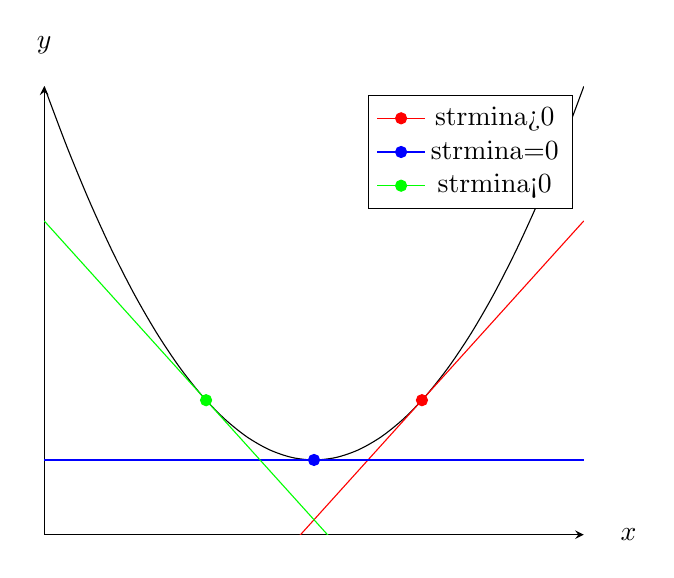
\begin{tikzpicture}
	\begin{axis}[xmin=-5, xmax=5, 
	ymin=-1, ymax=5, 
	xlabel=$x$, ylabel=$y$, 
	every axis x label/.style={
		at={(ticklabel* cs:1.05)},
		anchor=west,
	}, 
	every axis y label/.style={
		at={(ticklabel* cs:1.05)},
		anchor=south,
	}, 
	axis x line=left, 
	axis y line=left, 
	ticks=none]
	\addplot[color=black, smooth]{0.2*x^2};

	\addplot[color=red]{0.8*x - 0.8};
	\addplot[color=red, mark=*] coordinates {(2, 0.8)};

	\addplot[color=blue]{0};
	\addplot[color=blue, mark=*] coordinates {(0, 0)};

	\addplot[color=green]{-0.8*x - 0.8};
	\addplot[color=green, mark=*] coordinates {(-2, 0.8)};
	\legend{,,strmina>0,,strmina=0,,strmina<0}
	\end{axis}
	\end{tikzpicture}
\end{figure}
